\documentclass[conference]{IEEEtran}
\usepackage{times}

% numbers option provides compact numerical references in the text. 
\usepackage[numbers]{natbib}
\usepackage{multicol}
\usepackage[bookmarks=true]{hyperref}
\usepackage{booktabs}
\usepackage{amsmath}
\usepackage{color}
\usepackage{graphicx}

\newcommand{\todo}[1]{{\color{red} \textbf{{[TODO:}} {\em #1}\textbf{]}}}

\begin{document}

% paper title
\title{Decision Transformer for \\Robot Imitation Learning}
%OR Return Conditioned Robotic Imitation Learning with Decision Transformers for Robomimic Benchmarking
% You will get a Paper-ID when submitting a pdf file to the conference system
% \author{Alex Chandler, Jake Grigsby, and Omeed Tehrani}
\author{
    Alex Chandler \\ alex.chandler@utexas.edu \\ {University of Texas at Austin} 
   \and Jake Grigsby \\ grigsby@cs.utexas.edu \\ {University of Texas at Austin} 
   \and Omeed Tehrani \\ omeed@cs.utexas.edu \\ {University of Texas at Austin} 
}

\maketitle

\IEEEpeerreviewmaketitle

\begin{abstract}
Reinforcement learning typically involves an agent interacting with an environment to achieve a maximum reward. Our project disregards the traditional approach of estimating policies and simplifies Reinforcement Learning to a sequence modeling problem that can effectively be solved by the Transformer architecture. Our project extends the capabilities of the initial Decision Transformer (DT) \cite{decisiontransformer} to learn from mixed-quality input data. Our modified Decision Transformer quantifies the benefit of return-conditioned imitation learning on mixed-quality data by leveraging the robomimic datasets. We show that our Decision Transformer significantly outperforms standard behavioral cloning on mixed-quality data for the Lift and Can tasks. Overall, our Decision Transformer and semi-sparse reward function provide a new way to tackle the challenges of imitation learning with mixed-quality data.
\end{abstract}



\section{Introduction}
% Recent work has reformulated offline reinforcement learning as a sequence modeling problem that can be effectively solved with large Transformer models. Inspired by previous work on decision transformers, this paper re-implements Decision Transformer \cite{decisiontransformer} for use in the robomimic \cite{robomimic2021} benchmark. Transformers have taken over many subfields in ML, including Natural Language Processing, Natural Language Generation, and Computer Vision. We are motivated by the success of GPT-x, BERT, and other large language models outside of robotics. We evaluate our trained policies on two simulated manipulation tasks in robomimic \cite{robomimic2021} using low-dimensional states instead of image observations to reduce computational requirements. Our data source is a subset of the datasets included in the robomimic benchmark that includes large machine-generated data. Each task has multiple offline datasets based on quality; our focus is to have a decision transformer learn from mixed settings containing both novice and expert demonstrations, as this is where Decision Transformer's return-conditioning should provide the biggest advantage by filtering out failed attempts. We implement a custom version of the decision transformer model for robomimic data focused on continuous action spaces. We experiment with a simpler input embedding that saves compute by shortening the input sequence. We evaluate and analyze the average return of the policy in the test environment. We evaluate the policy's ability to replicate multiple levels of desired return. We measure the average success rate of $50$ evaluation roll-outs. Our model outperforms behavioral cloning accuracy on the Lift and Can tasks trained on mixed-quality data. All of our transformer code and experiments are available through GitHub.



Robot imitation learning methods use supervised learning to mimic the actions necessary to complete complex tasks. This process typically involves a time-consuming cycle of collecting and filtering high-quality human demonstrations. In order to increase data availability and ease of use, we would like to learn from sub-optimal demonstrations. Sources of sub-optimal data may include inexperienced human teleoperators, scripted agents, or past versions of our own learning-based policy. Learning from fixed datasets of mixed-quality experience is often studied in offline Reinforcement Learning (RL) \cite{levine2020offline}. Despite a recent surge in research interest, offline RL remains challenging in practice, and it can be difficult to develop a method that achieves real-world results. Our project focuses on the Decision Transformer \cite{decisiontransformer} - a simple and powerful alternative to RL algorithms that replaces brittle dynamic programming and policy gradients with standard sequence modeling. Like more traditional offline RL methods, Decision Transformer (DT) can learn from mixed-quality demonstrations by conditioning action outputs on the total return of each trajectory. DT policies can then imitate high-quality data while gathering extra information about the task by modeling low-quality demonstrations. At test-time, we can specify an expert-level target return and deploy a policy with the performance of expert imitation learning without the need for expensive curated datasets. DT reduces offline RL to a training routine that resembles sequence models in supervised learning. There is optimism that we can leverage diverse datasets and large network architectures similar to those that have been successful in domains like natural language processing to improve generalization in robot decision-making. 

    \par In this project, we implement a custom version of the Decision Transformer focusing on continuous action spaces and stochastic policies. We evaluate our implementations' ability to learn from mixed-quality data using two simulated domains from the robomimic benchmark \cite{robomimic2021} that provide machine-generated and expert demonstrations. We study the impact of several design decisions on task success rates, including model size, policy parameterization, and context sequence lengths. Results demonstrate that our DT implementation significantly outperforms naive Behavioral Cloning in this mixed-quality and multi-modal setting. We also discuss some limitations of our work and opportunities for future improvement on the robomimic benchmark. The code for this project is open-sourced and available on GitHub to enable future research\footnote{\url{https://github.com/jakegrigsby/robomimic-decision-transformer}}.





\section{Background and Related Work}
\label{sec:relatedwork}

\subsection{Reinforcement Learning}
In the Reinforcement Learning  setting considered in this paper, an agent interacts with an environment in order to maximize a reward signal. At each timestep $t$, the agent perceives a state $s_t$ and selects an action $a_t$, leading to a new state $s_{t+1}$ and a reward $r_t$. The agent's decision-making strategy is defined by its policy $\pi$, which maps states to a distribution over actions $\pi(a_t \mid s_t)$. Our goal at every timestep is to maximize the cumulative sum of rewards until some time limit of $H$ steps, also known as the return. We will use the term ``return-to-go" (RTG) to refer to the return after a specific timestep $t$. The RTG at timestep $t$ is denoted $\hat{R}_t = \mathop{\sum}_{i=t}^{H}r_i$. Decision Transformer computes RTG values in hindsight from an offline dataset and uses them to differentiate between low and high-quality demonstrations.

\subsection{Offline Reinforcement Learning}
Offline RL \cite{levine2020offline} studies decision-making from fixed datasets of prior experience. Unlike standard ``online" RL, offline agents cannot explore the environment to gather new information about the task. Instead, offline methods attempt to stitch together optimal decision-making strategies from datasets of sub-optimal data to match or exceed the performance of the policies that generated the training dataset. Offline algorithms often have to confront technical challenges 
arising from situations our dataset does not cover. For example, methods such as CQL \cite{kumar2020conservative}, CRR \cite{NEURIPS2020_588cb956}, and BCQ \cite{fujimoto2019off} restrict their policies' action choices to those present in the dataset in order to avoid out-of-distribution optimization issues. Model-based methods such as MOPO \cite{yu2020mopo} explicitly penalize actions that lead to uncertain states. The ultimate goal of offline RL is to develop a scalable way to reuse data and deploy RL to real-world tasks, where data collection is expensive or unsafe. Examples include self-driving cars, healthcare, and real-world robotics \cite{levine2020offline}. However, current methods can be difficult to develop and tune without the ability to evaluate policies in the test environment. Recent research has worked to simplify techniques \cite{fujimoto2021minimalist} and develop a repeatable workflow \cite{kumar2021workflow} for new applications.


\subsection{Robomimic}
Robomimic\footnote{\url{https://github.com/ARISE-Initiative/robomimic}} \cite{robomimic2021} is a framework for offline robot learning from demonstrations as a part of the Advancing Robot Intelligence through Simulated Environments (ARISE) Initiative. Robomimic includes a unique collection of standardized human-collected and machine-generated datasets for offline RL and imitation learning. The benchmark currently supports several simulated manipulation tasks including ``Lift", ``Can", ``Tool Hang", and ``Square Transport". These tasks use the robosuite simulator \cite{zhu2020robosuite} to enable affordable access to offline robotics research. These simulated environments can be configured to use low-dimensional proprioceptive states instead of high-dimensional rendered images. Robomimic also includes real-robot variants of similar tasks with camera-based observations.

Robomimic divides each task's offline dataset into several categories based on demonstration quality and extensively benchmarks behavioral cloning (BC) and offline RL algorithms. The results suggest that learning from a mixture of human datasets can be challenging because of the varying proficiency and strategies of multiple demonstrators. Each teleoperator solves the same task slightly differently, which leads to multi-modality even in simple tasks; this effect would likely be more problematic in the kinds of long-horizon tasks we would eventually like robots to solve. The robomimic authors find that offline RL methods can be challenging to use in practice and are often outperformed by simpler BC techniques. In particular, they find that the strongest baseline is a memory-equipped BC policy that uses a Recurrent Neural Network (RNN) to process sequences of observations. This BC-RNN baseline improves action prediction by using its memory of past timesteps to address the multi-modality of mixed human demonstrators. However, BC-RNN still struggles when the dataset contains low-quality demonstrations because it learns to imitate all of the decisions in the training set as one unified policy.
% The eight tasks have been extensively tested on 6 offline learning algorithms BC, BC-RNN, HBC, BCQ, CQL, IRIS. The tasks have also been tested in 2 observation spaces: 1) low-dimensional agents with ground truth and 2) image agents that receive camera observations. Information and the code repository for robomimic are available through GitHub\footnote{\url{https://github.com/ARISE-Initiative/robomimic}}. 

% More formally known as "Behavioral Cloning with Recurrent Neural Network policy", BC-RNN enables us to model temporal correlations in decision-making \cite{robomimic2021}. In one of the core lessons from robomimic, it was found that methods that make decisions based on history, such as BC-RNN, tend to outperform other methods, especially on human datasets. \cite{robomimic2021}. RNNs, however, are computationally intensive due to their un-parallelizable architecture, and they are susceptible to the exploding gradient problem. Additionally, they are not as good as transformers at handling long-term dependencies. Transformers, on the other hand, have recently been found to generate higher-quality output than RNN sequence-to-sequence models while demanding less computation \cite{transformer}. These issues with RNNs are some of the leading motivations for us to use transformer architecture.

% The variability of human behavior presents a significant challenge to imitation learning algorithms, like BC-RNN, attempting to learn from mixed-quality data. Imitation learning algorithms struggle when trained from multiple human demonstrators, as the algorithms must be able to accurately capture and generalize from the diverse ways in which different individuals may perform a given task. Furthermore, the varying goals and objectives of these individuals can make it difficult for the algorithm to determine the appropriate action to take in a given situation. This can lead to suboptimal performance, particularly when the presence of multiple demonstrators makes it difficult for the algorithm to identify the most important or relevant actions to learn from.


\subsection{Outcome-Conditioned Behavioral Cloning}
Recent work has looked to simplify offline RL by creating similarities to supervised learning techniques in related fields like natural language processing and computer vision. One promising approach adds the return-to-go of the offline trajectory as an extra input to a BC algorithm: $\pi(a_t \mid s_t, \hat{R}_t)$. This lets the policy differentiate between high and low-quality experiences during training. Low-quality data helps increase the size of the training set and may provide some valuable knowledge of the task. However, we can replicate only the high-quality actions at test-time by specifying an expert-level target return $\hat{R}_0$. Return-conditioned behavior cloning can often match or outperform more complicated RL algorithms \cite{rvs, rcp, brandfonbrener2022does}. The idea of conditioning behavioral cloning on the quality of the demonstration datasets also appears as ``Upside Down RL" \cite{udrl_idea, udrl_implementation}. The method has conceptual similarities to goal-conditioned reinforcement learning \cite{nair2018visual, andrychowicz2017hindsight}, which we can reformulate as a supervised learning problem conditioned on states instead of returns \cite{eysenbach2022imitating, ghosh2019learning}.

\subsection{Decision Transformers}
The Transformer architecture \cite{transformer} uses an attention mechanism to process sequences without convolution or recurrence. Originally utilized for machine translation in natural language processing, the Transformer architecture has since appeared in state-of-the-art models for tasks across nearly every domain in machine learning. Transformers rely on a scaled dot-product attention mechanism that enables the representations of each timestep to interpret patterns across all the preceding timesteps in the sequence. Transformers are highly compatible with GPU parallelization and can learn complex temporal dependencies. Transformers are generally known to outperform RNN models while being more computationally efficient.

Decision Transformer \cite{decisiontransformer} is an algorithm that combines the simplicity of return-conditioned BC with the performance of large Transformer networks. The Trajectory Transformer \cite{trajectorytransformer} is a concurrent work that adds language modeling techniques like beam search to RL. Additional extensions of the Decision Transformer concept include online fine-tuning \cite{online_decisiontransformer}, few-shot prompting \cite{xu2022prompting}, and applications to stochastic environments \cite{esper}. Finally, Gato \cite{gato} uses a similar architecture and tokenization scheme to Decision Transformer, although on a much larger scale and without return-conditioning.

\section{Method}
\label{sec:method}


\subsection{Data}

Our data is collected and processed from the robomimic dataset \cite{robomimic2021},  providing us with a large-scale dataset of robot demonstrations for a variety of tasks. The dataset includes three types of data: machine-generated (MG), proficient-human (PH), and multi-human (MH). The machine-generated data is generated by state-of-the-art reinforcement learning agents and is of varying quality, ranging from sub-optimal to high-quality. The proficient-human and multi-human data are demonstrations from teleoperators with varying levels of proficiency.

In this work, we focus on two tasks from the robomimic dataset: Lift and Can. The Lift task involves a robot lifting a cube, while the Can task involves picking up a can and placing it in the correct bin. These tasks were chosen because robomimic provides a large number of machine-generated (low-quality) demonstrations for those two tasks, which highlights the problem of learning from mixed datasets. To evaluate our approach, we create a fourth dataset for each task. This ``All" dataset category is a challenging combination of the machine-generated, multi-human, and proficient-human data. Because there is much more MG data than human demonstrations, the ``All" dataset is weighted towards lower-quality data, making it an interesting challenge for our purposes. Using this dataset, we can test DT's ability to learn from both high-quality and low-quality demonstrations. The Lift environment is shown in Figure \ref{fig:task_lift} and the Can environment is shown in Figure \ref{fig:task_can}. 

\begin{figure}
\centering
\begin{minipage}{.24\textwidth}
  \centering

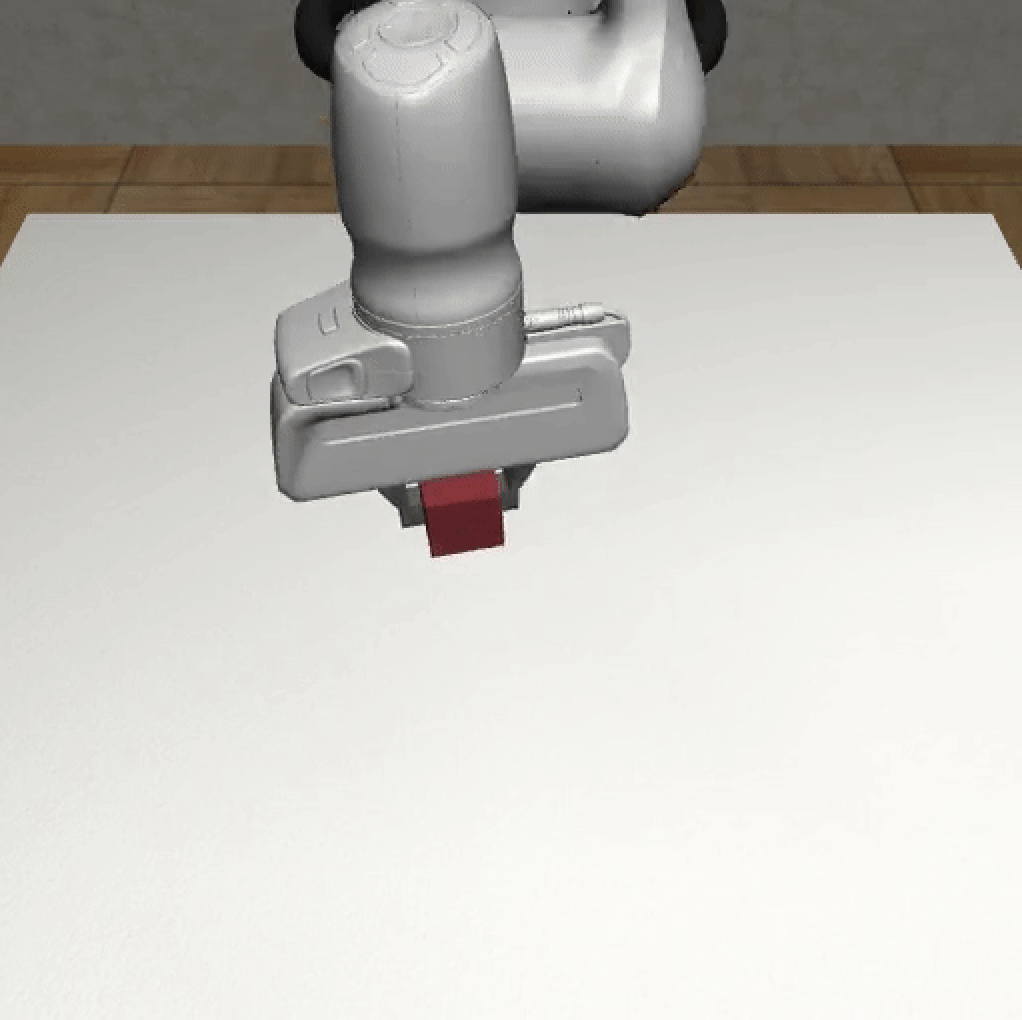
\includegraphics[width=.95\linewidth]{figs/task_lift.png}
    \centering
   \caption{The Lift task, where \\the goal is to pick a red cube \\off of the tabletop.}
  \label{fig:task_lift}
\end{minipage}%
    \centering
\begin{minipage}{.24\textwidth}

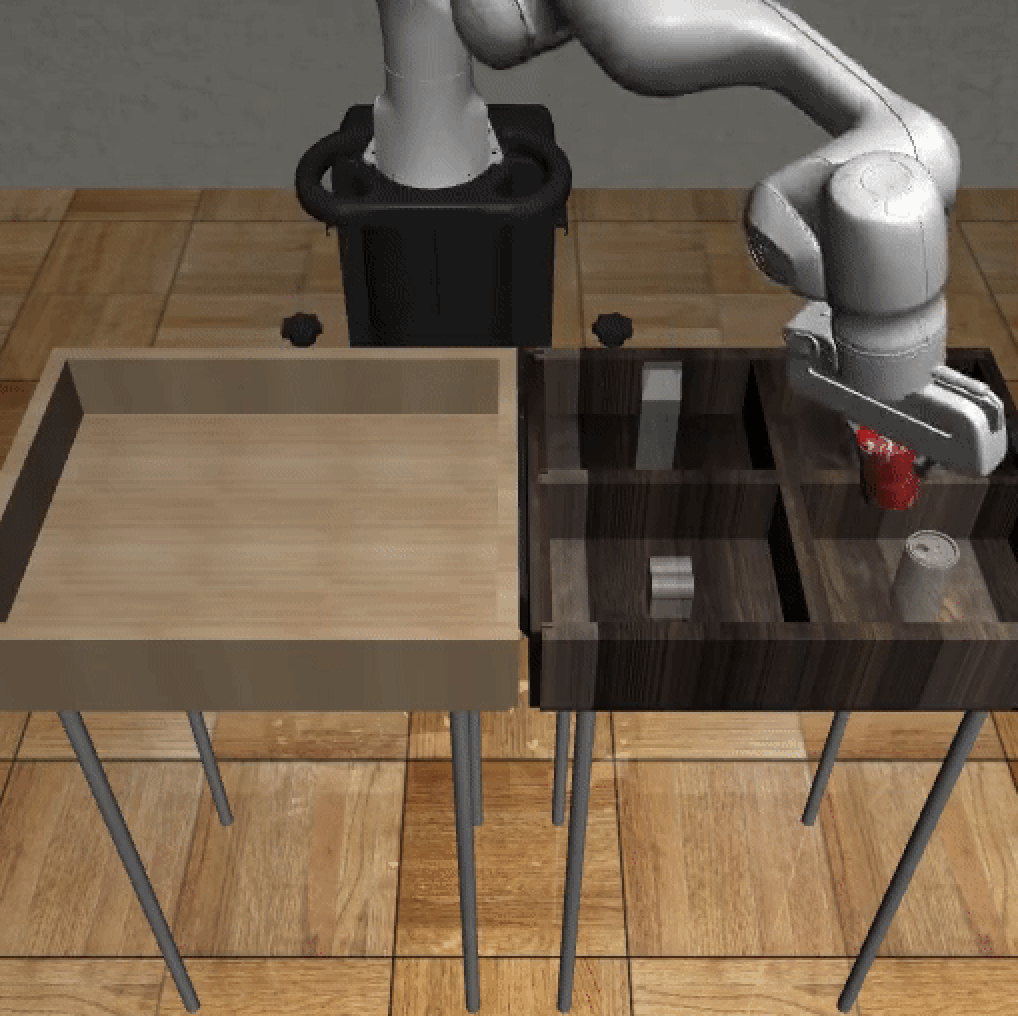
\includegraphics[width=.95\linewidth]{figs/task_can.png}
  \centering
  \caption{The Can task, where the goal is to pick up the red can and deposit it in the proper container.}
  \label{fig:task_can}
\end{minipage}
\end{figure}



\subsection{Semi-Sparse Reward Function}
The offline datasets in the original robomimic study use a binary reward function where the agent receives a reward of $1$ for successful completion of the task and $0$ at all other timesteps. Decision Transformer uses dense reward functions to differentiate between many different modes of policy quality \cite{decisiontransformer}. Therefore, our first step was to assign a more dense reward signal to robomimic's manipulation tasks. The robomimic codebase does provide an option to relabel datasets with robosuite's dense reward function. However, we found that the resulting rewards were not correlated with the quality of the dataset. In the Lift task dataset, for example, the proficient-human demos had the highest success rate but the lowest return values, while machine-generated data had the lowest success rate but the highest returns. This was a result of the worse quality demonstrations compensating for their low reward per timestep by taking much longer to solve the task, leading to a higher total return. To address the issue, we manually changed the reward function to include a semi-sparse success bonus. We added a large positive reward upon completion of the task which decreases with every timestep. Let $r_t^{\text{robomimic}}$ be the original dense reward term provided by the robomimic dataset at time $t$, and $d_t$ be a binary ``done" flag where $d_t = 1$ indicates successful task completion. We define a new reward term $r_t^{\text{DT}}$:
\vspace{-2.5mm}
\begin{align}
    r_t^{\text{DT}} = r_t^{\text{robomimic}} + d_t \max(500 - t, 0) 
    \label{eq:rt}
\end{align}

The success bonus decreases to zero after $500$ timesteps, which is the maximum length of the robomimic tasks. We relabel the offline dataset using Equation \ref{eq:rt}, and modify the reward function in the environment simulator for evaluation. This design lets our DT learn from a wide range of target values and improve its understanding of the quality of the sequence data, even in the presence of low-quality data.

\subsection{Decision Transformer Architecture}

% 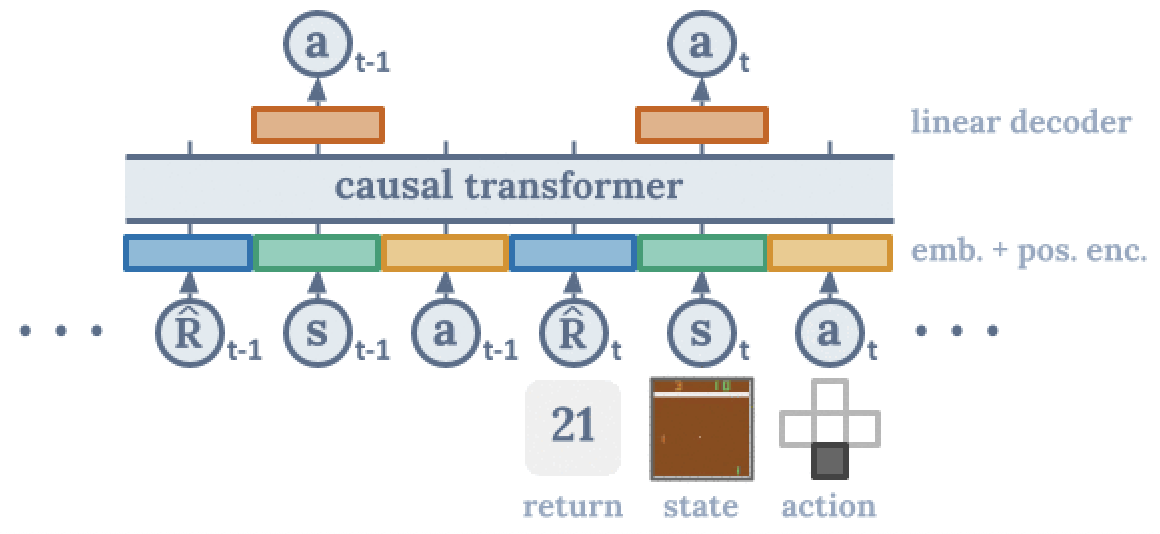
\includegraphics[width=0.5\textwidth]{figs/original.png}

 \noindent Our implementation is a modification of the original Decision Transformer architecture. The input format is a \textit{context sequence} of up to $k$ \textit{tokens}, where $k$ is the context length. Each token is a vector that concatenates a state $s_t$, return-to-go $\hat{R}_t$, and the previous action $a_{t-1}$\footnote{The first timestep of every trajectory is missing a previous action ($a_{-1}$), which we define as a zero vector.}. All sequences are padded to a length of $k$. The resulting sequence is projected to the embedding dimension of the Transformer architecture with a two-layer feedforward network. Transformers are permutation-invariant and require a position encoding to interpret the order of input tokens. The original Transformer \cite{transformer} used a hardcoded sinusoidal embedding. Instead, we randomly initialize embedding vectors for each of the $k$ position indices and train them alongside the rest of the model. This solution is more popular in domains with continuous inputs such as Vision Transformers \cite{dosovitskiy2020image}. The ($s, a, \hat{R}$) and position embeddings are summed together and form the input sequence of the core Transformer architecture. Our input format is a slight departure from the original DT, which embedded states, actions, and RTGs as separate consecutive tokens. Our concatenated version simplifies the implementation and position embedding while saving compute by reducing the overall sequence length by a factor of $3$.
 
 % This allows us to reduce the length of the sequences and the overall computational requirements of the model, as we only need to store a single token for each state-action pair instead of separate values for the state-action and return in the original decision transformer architecture.
 
 The embedded sequence of tokens is then fed into a causal Transformer, which uses a self-attention mechanism to model the dependencies between the tokens. We use a Pre-Norm Transformer \cite{xiong2020layer} architecture, which shifts the location of the layer normalization component to the residual branch. This is thought to improve stability early in training and enable deeper networks. The output of the Transformer is a sequence with the same dimensions as the embedded input. After a final normalization layer, this sequence is projected by a two-layer feedforward network into the dimension of the action distribution. The original DT uses a deterministic policy that outputs the action vector directly and is trained with mean squared error. We are focused on manipulation tasks with highly multi-modal demonstrations that would be difficult to model with a deterministic policy. Instead, our network generates the parameters of a stochastic distribution over actions. We implement a Gaussian policy with independent parameters for each dimension of the action space - a common default in the RL literature (e.g., \cite{schulman2017proximal, haarnoja2018soft}). We also add a Gaussian Mixture Model (GMM) policy based on robomimic that adds extra parameters in order to better represent multi-modal action distributions. We use the GMM parameterization with $5$ modes by default, and compare the two policy types in the Section \ref{sec:experiments}. A high-level summary of our DT model is depicted in Figure \ref{fig:arch}.
 
 
 % By using a multi-modal stochastic policy, our approach is able to capture the uncertainty and variability of continuous actions, resulting in improved performance compared to the deterministic policy used in the original paper \cite{decisiontransformer}.

% It is important to note that the original decision transformer uses a deterministic policy, where the action taken at each time step is determined by the current state and the previous actions with no uncertainty. In contrast, we train a multi-modal stochastic policy, where the action taken at each time step is modeled as a probability distribution over a range of possible actions. This allows us to better model continuous actions, where the exact action taken may vary within a certain range: 

% \begin{align}
% \pi(a|s) = P(A = a | S = s)
% \end{align}


% By using a multi-modal stochastic policy, our approach is able to capture the uncertainty and variability of continuous actions, resulting in improved performance compared to the deterministic policy used in the original paper \cite{decisiontransformer}. See Figure \ref{fig:arch} for more details.  \\

\begin{figure}[h!]
    \centering
    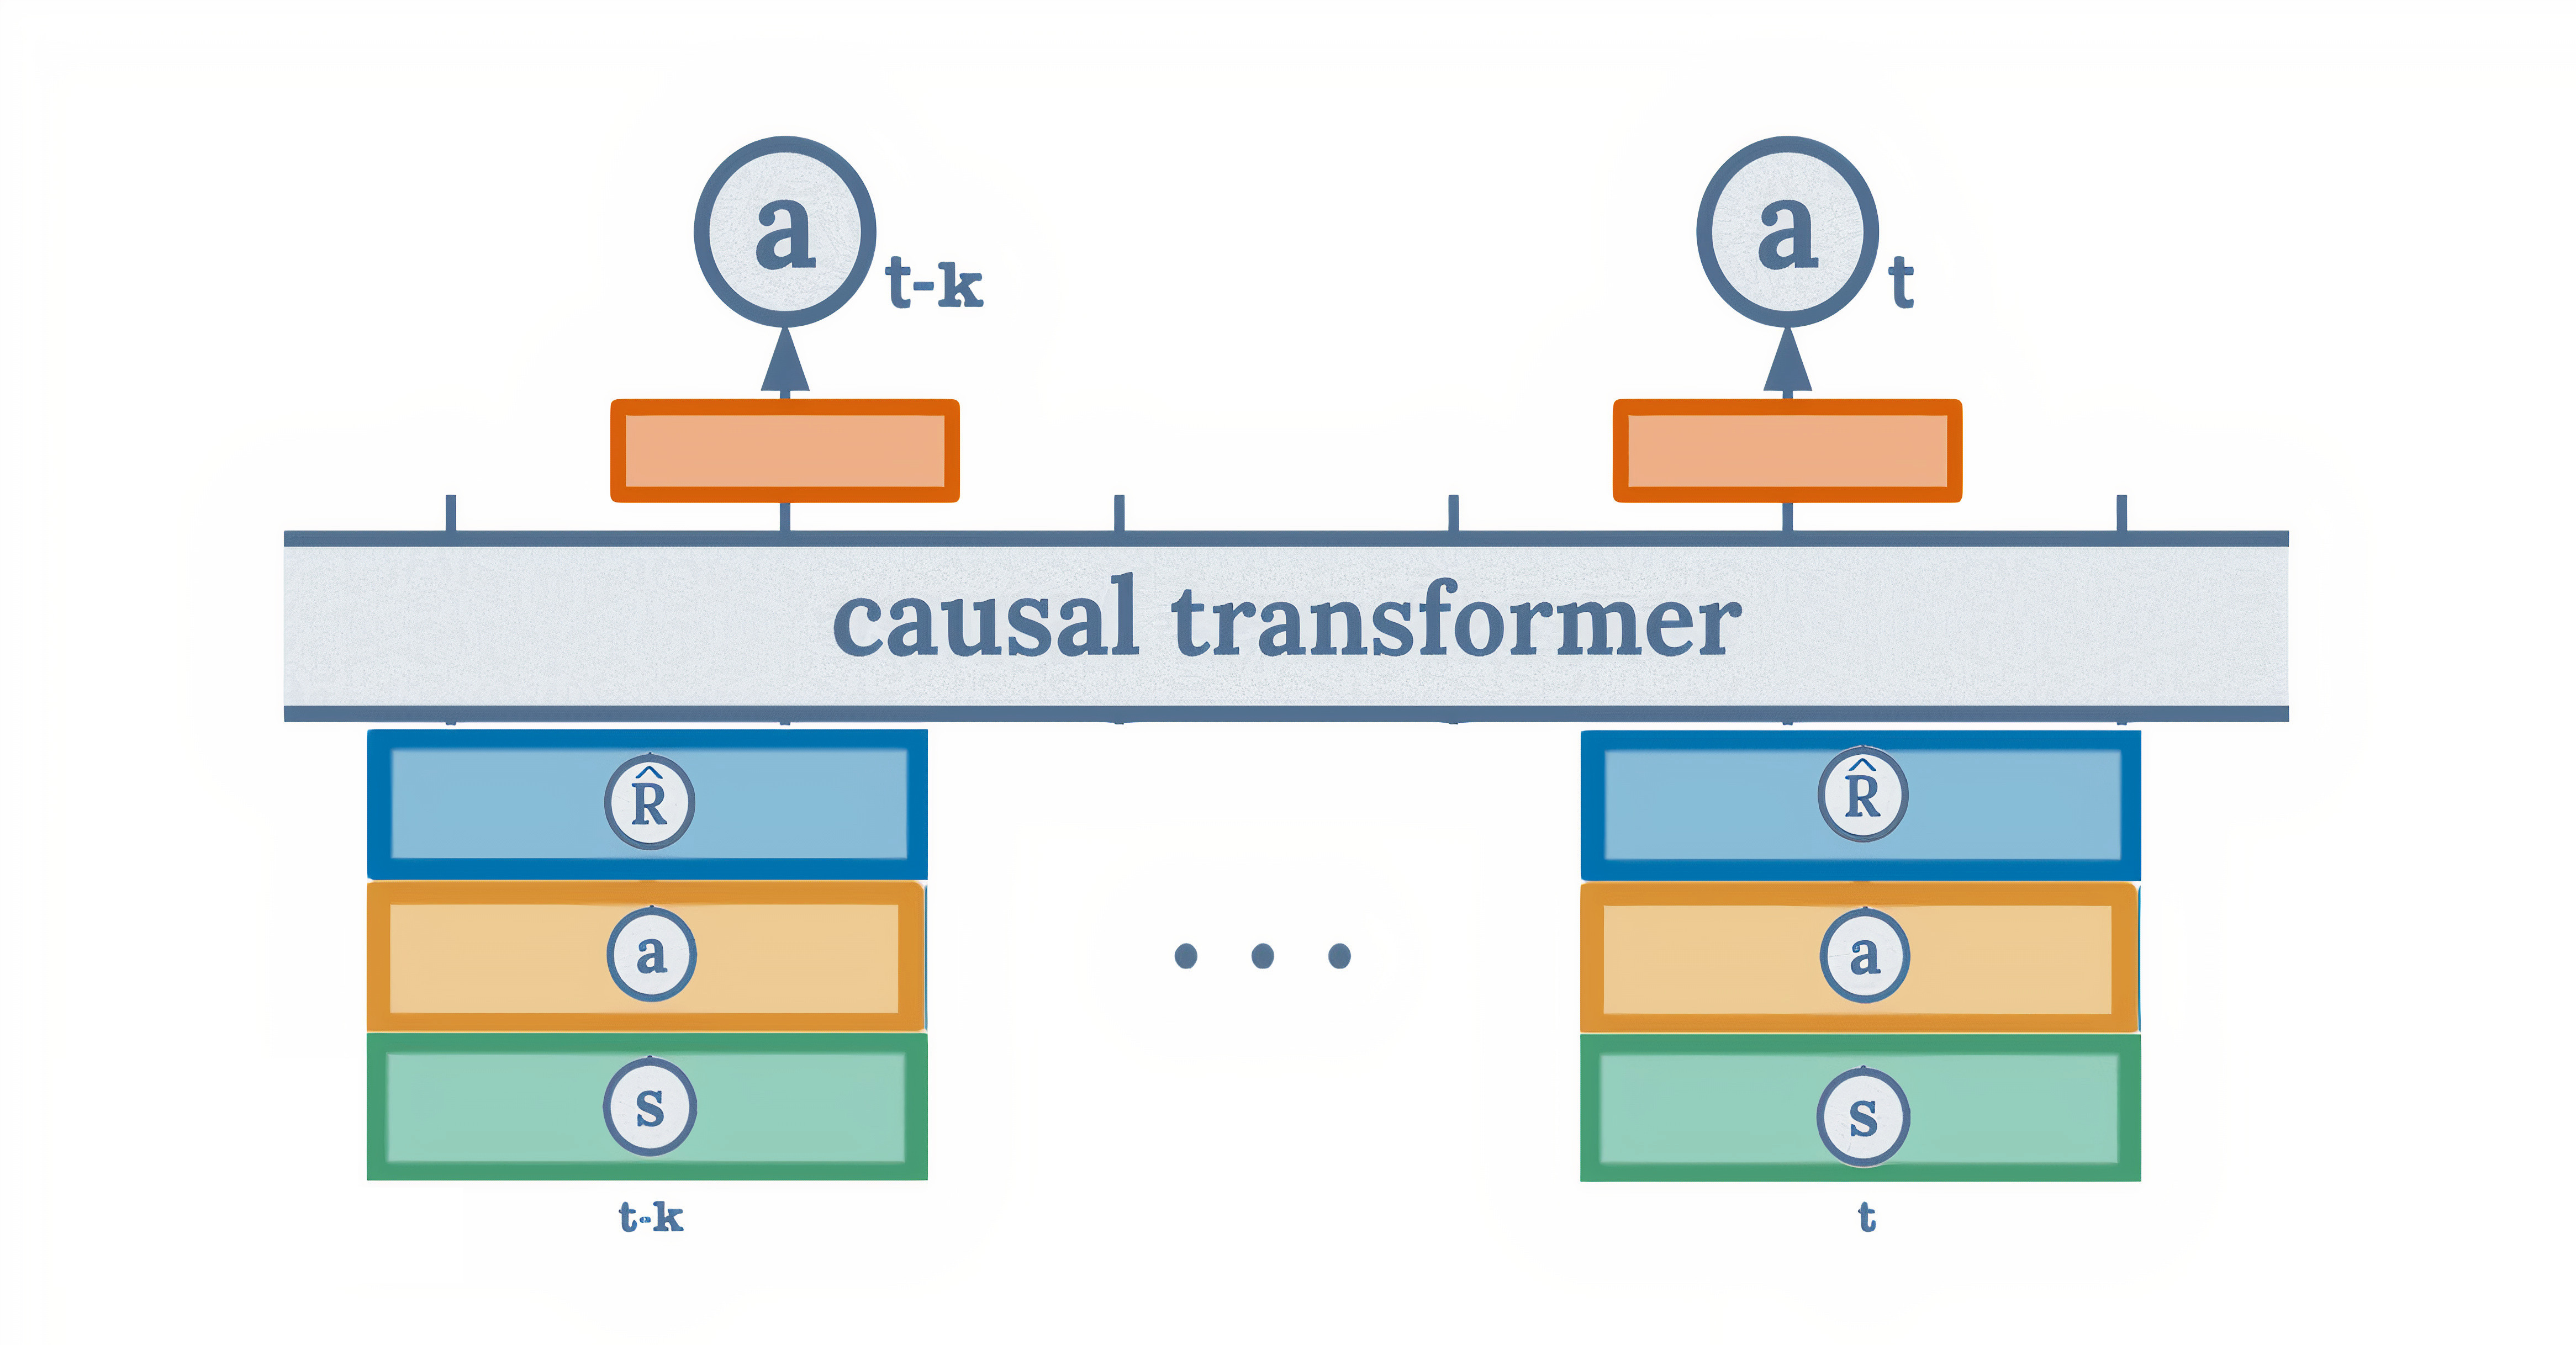
\includegraphics[width=.45\textwidth]{figs/arch.jpg}
    \caption{Our Decision Transformer architecture, with states, actions, and return-to-go values concatenated into one token. DT maps a context sequence of $k$ tokens to a sequence of $k$ action distributions.}
    \label{fig:arch}
\end{figure}


\subsection{Training}
Decision Transformer uses a standard sequence modeling objective and training loop. This can greatly simplify its implementation relative to many techniques in offline RL, where best practices are an open research topic \cite{kumar2021workflow}. We optimize our network parameters $\theta$ to maximize the probability of true actions in the dataset ($\mathcal{D}$) given the sequence of $k$ previous states, actions, and RTG values:

\vspace{-5mm}
\begin{align}
    c_t &:= (s_t, a_{t-1}, \hat{R}_t) \nonumber \\
    \theta^{\ast} &:= \mathop{\mathbb{E}}_{a_t, c_{t}, \dots, c_{t-k} \sim \mathcal{D}}[-\text{log}\pi_{\theta}(a_t \mid c_{t}, \dots, c_{t-k})]
    %\theta^{\ast} &:= \mathop{\text{argmin}}_{\theta}  \mathop{\mathbb{E}}_{a_t, c_{t-1}, \dots, c_{t-k} \sim \mathcal{D}}[-\text{log}\pi_{\theta}(a_t \mid c_{t-1}, \dots, c_{t-k})]
    \label{eq:loss}
\end{align}

We use several empirical best practices from the wider Transformer literature to stabilize training, including the AdamW optimizer \cite{loshchilov2017decoupled} and a linear learning rate warm-up for the first two thousand gradient steps \cite{transformer}. The batch size is fixed at $256$. Training is performed on a single NVIDIA GeForce RTX-3090 and takes roughly $6$ hours depending on model size. Much of the training time is consumed by evaluation rollouts in the simulated environments which are comparatively slow. We perform the evaluation in parallel across $8$ independent environments, batching and padding the sequences into one forward pass of the Transformer.



\section{Experiments}
\label{sec:experiments}

\par In this section, we explore the challenges of action and return conditioned imitation learning and provide results for the Can and Lift tasks. We investigate the effects of introducing inaccuracies at test-time by conditioning the policy on its own slightly inaccurate history of actions and return-to-go values. Our experiments show that these inaccuracies can lead to lower task success rates for Decision Transformers (DT) compared to behavior cloning (BC) baselines. We then train DT models with various context sequence lengths on the more difficult "All" data setting of the Can task and show that longer context sequences improve prediction accuracy. Finally, we compare DT against BC baselines on the mixed-quality ``All" dataset, demonstrating the effectiveness of DT's return-conditioning and context sequences for imitation learning in complex environments.

\subsection{Understanding the Challenges of Action and Return-Conditioned Imitation Learning}
\label{sec:challenges}
Decision Transformers condition their outputs on a fixed-length history of previous actions, return-to-go scalars, and observations. While this may help differentiate between the various demonstrators in a mixed-quality dataset, it also introduces new opportunities for distributional shifts during evaluation: at test-time, the policy is conditioned on the history of its own (slightly inaccurate) actions and return-to-go values. These inaccuracies can compound over the length of a trajectory, potentially causing DT to achieve a lower task success rate than a BC baseline. As a first step, we investigate this effect on the Can placement task using only the highest quality dataset of human demonstrations (PH). In this setting, DT's ability to learn from mixed-quality data is less relevant. We use context lengths of one to compare directly against BC, meaning that the input to a DT model during evaluation is the most recent state, action, and return-to-go. We can optionally hide the action and/or RTG information. Hiding actions and RTGs recover the simple BC baseline, and a context length of one makes the attention component of the Transformer redundant. 

Success rates are measured by pausing training and evaluating the current policy in the robomimic environment simulator. The success rates of several ablations of DT input format over the course of training are plotted in Figure \ref{fig:can_ph_success_rates}. While standard BC matches the performance of the demonstrations and the original robomimic baselines, DT variants that introduce action and RTG inputs can struggle to achieve expert results. Increasing model size appears to improve performance by outputting more accurate actions and being more robust to variations in the input.

\begin{figure}
    \centering
    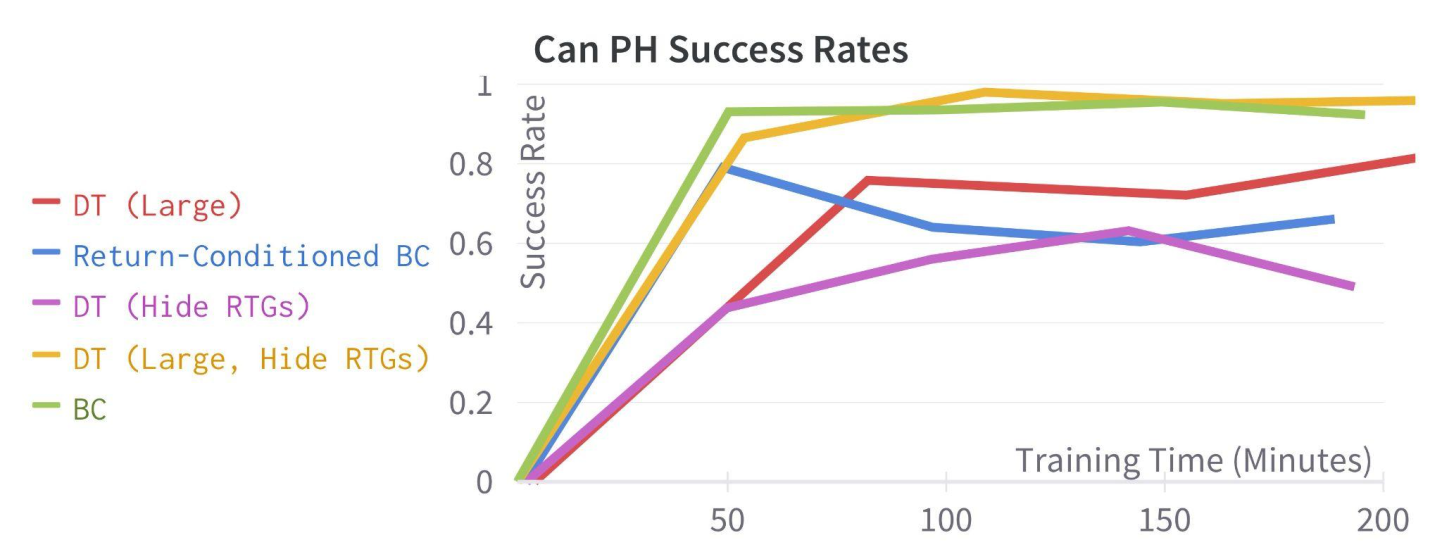
\includegraphics[width=\linewidth]{figs/can_ph_success_rates.png}
    \caption{Success rate of ablations of the DT input format in the Can task using only the highest quality PH data. ``Large" policies double the networks' embedding and feedforward dimensions.}
    \label{fig:can_ph_success_rates}
\end{figure}

\subsection{Decision Transformer on Can and Lift Tasks}
Although action and RTG inputs may harm performance at test-time, our next experiment investigates whether DT's sequence inputs improve the accuracy of action predictions during training. We train identical DT agents with context lengths of $3, 10$ and $20$ on the more difficult ``All" data setting of the Can task. We would expect longer context sequence lengths to improve prediction accuracy by providing more information on the quality and action choices of the demonstrator that created each training sequence. The negative log-likelihood training loss (Equation \ref{eq:loss}) for the three models is plotted in Figure \ref{fig:can_all_train_loss}. Despite equal model sizes, regularization, and optimization settings, DT's fit of the training data improves with context sequence length. 

\begin{figure}
    \centering
    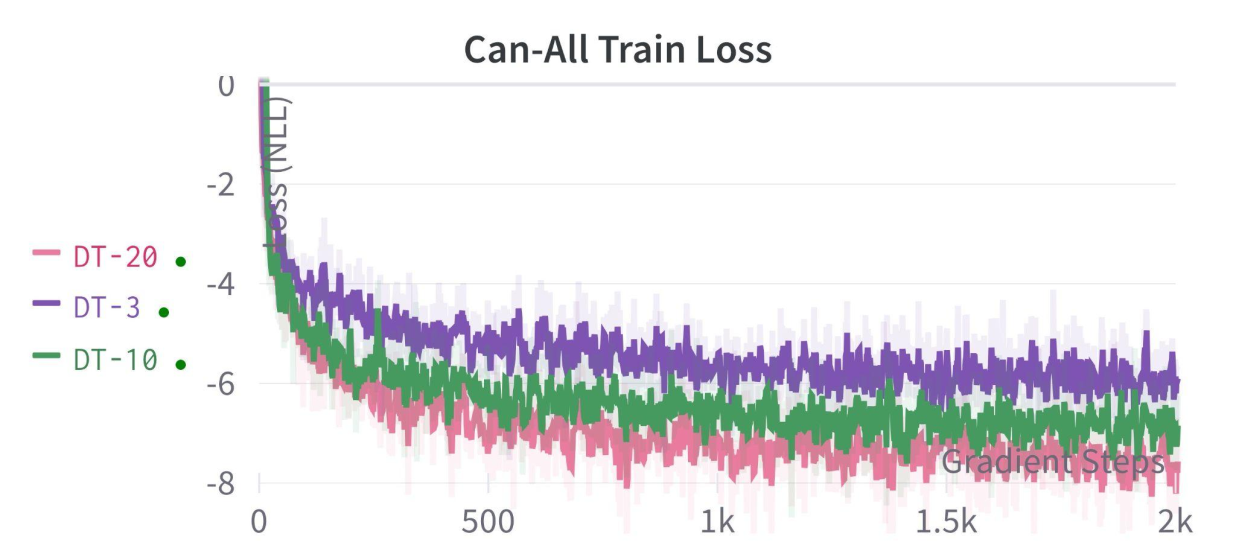
\includegraphics[width=\linewidth]{figs/can_all_train_loss.png}
    \caption{Training Loss of DT with context lengths of $3, 10$ and $20$. Longer context sequences improve action predictions by resolving ambiguity about which demonstrator is being imitated.}
    \label{fig:can_all_train_loss}
\end{figure}

Next, we conduct a larger-scale evaluation of DT with various context lengths and policy types. We compare against simpler BC baselines on the mixed-quality ``All" dataset types consisting of both low-quality machine-generated data and high-quality human demonstrations. The results for the Lift task are shown in Table \ref{tbl:liftresults}, where DT-$k$ denotes our Decision Transformer model with a context sequence of length $k$. Because DT is conditioned on the return-to-go values of its training data, we need to select a target return to imitate at test-time. We settle on the simple heuristic of finding the $95$th percentile of the returns in the training dataset. We explore this choice further in Section \ref{sec:expreturnsweep}. The \textit{Naive BC} method uses a Gaussian policy without context sequences or return-conditioning and achieves a success rate of just $35\%$ - highlighting the challenges of imitation learning from mixed-quality datasets with multiple demonstrators. For comparison, the original robomimic BC results achieve a success rate of $100\%$ using the PH data and $65\%$ from the lowest-quality MG data. We replicate these experiments with our codebase and report success rates of $99\%$ for \textit{Naive BC} on PH data. This suggests that learning from the mixed ``All" dataset is more difficult than learning from any of its sub-components as a result of multi-modality. DT uses return-conditioning to filter dataset quality and context sequences to resolve multi-modality. As a sanity check, we train DT-$1$ on the PH data with $100\%$ success. DT-$1$ still sees a decrease in performance on the ``All" dataset but uses its return-conditioning to improve significantly on the BC baseline with a success rate of $85\%$. By extending the context sequence to $20$ timesteps, DT-$20$ can further improve to $94\%$.

\begin{table*}[]
\centering
\caption{\textbf{Lift-All Results}}
\resizebox{.8\textwidth}{!}{
\begin{tabular}{@{}lccccccc@{}}
\toprule
 & Naive BC & \begin{tabular}[c]{@{}c@{}}BC +\\ Action Inp.\end{tabular} & \begin{tabular}[c]{@{}c@{}}DT-1 \\ (PH Only)\end{tabular} & DT-1 & DT-3 & DT-10 & DT-20 \\ \midrule
Success Rate (\%) & 35 & 20 & \textit{100} & 85 & 92 & 92 & \textbf{94} \\
Return & 189 & 113 & \textit{463} & 397 & 428 & \textbf{433} & 421 \\ \bottomrule
\end{tabular}
}
\label{tbl:liftresults}
\end{table*}

Table \ref{tbl:canresults} shows the results of a similar experiment on the Can task. Although we successfully replicate the near-perfect success rate of the original robomimic results on the PH data, Naive BC once again fails ($14\%$) on our mixed dataset. The relative performance of the methods on Can is similar to Lift, although we find the return and action conditioning to have a negative impact on this task as noted in Section \ref{sec:challenges}. \hspace{7mm} DT-$3$ achieves the highest performance on Can-All with a task success rate of $81\%$. Further discussion of the challenges in recovering the $100\%$ success rate of the PH dataset with our Decision Transformer model is provided in Section \ref{sec:discussion}.



\begin{table*}[]
\centering
\caption{\textbf{Can-All Results}}
\resizebox{.8\textwidth}{!}{
\begin{tabular}{@{}lcccccc@{}}
\toprule
 & \begin{tabular}[c]{@{}c@{}}BC \\ (PH Only)\end{tabular} & Naive BC & \begin{tabular}[c]{@{}c@{}}BC + \\ Action Inp.\end{tabular} & DT-3 & DT-10 & DT-20 \\ \midrule
Success Rate (\%) & \textit{99} & 14 & 15 & \textbf{81} & 76 & 63 \\
Return & \textit{396} & 72 & 74 & \textbf{362} & 337 & 286 \\ \bottomrule
\end{tabular}
}
\label{tbl:canresults}
\end{table*}


\subsection{Ablations}
There are two key implementation details that affect the performance of the Decision Transformer which could benefit from further analysis. First is the size of the Transformer architecture. While massive multi-billion parameter Transformers have been essential for progress in language modeling \cite{brown2020language} when learning from internet-scale datasets, recent applications of Transformers to RL and robotic control problems have preferred much smaller model sizes \cite{shafiullah2022behavior, decisiontransformer, cui2022play}. We compare the performance of the larger Transformer used in the main Can-All experiments (Table \ref{tbl:canresults}) - which used an embedding dimension of $512$, a feedforward dimension of $2048$, and $4$ Transformer layers - with a smaller architecture of $3$ layers with embedding dimension $200$ and feedforward dimension $800$. The smaller architecture is the same as was used for the easier Lift-All experiments (Table \ref{tbl:liftresults}). The results are shown in Table \ref{tbl:modelsizes}. The larger model appears to provide a meaningful improvement in performance across all three context lengths. Because expert human demonstrations are expensive to collect, related work in Transformers for robotic imitation learning uses architectures much smaller than even our ``Small" model to prevent overfitting. DT's return-conditioning offers a promising way to make use of diverse experiences and benefit from the generalization of large networks.

\begin{table}[h!]
\caption{\textbf{DT Network Sizes on Can-All}}
\resizebox{\columnwidth}{!}{
\begin{tabular}{@{}lccccccc@{}}
\toprule
 & \begin{tabular}[c]{@{}c@{}}DT-3 \\ (Large)\end{tabular} & \begin{tabular}[c]{@{}c@{}}DT-10 \\ (Large)\end{tabular} & \begin{tabular}[c]{@{}c@{}}DT-20 \\ (Large)\end{tabular} & \begin{tabular}[c]{@{}c@{}}DT-3 \\ (Small)\end{tabular} & \begin{tabular}[c]{@{}c@{}}DT-10\\  (Small)\end{tabular} & \begin{tabular}[c]{@{}c@{}}DT-20 \\ (Small)\end{tabular} & \begin{tabular}[c]{@{}c@{}}DT-3 \\ (Large, Gaussian)\end{tabular} \\ \midrule
Success Rate (\%) & \textbf{81} & 76 & 63 & 65 & 57 & 61 & 66 \\
Return & \textbf{362} & 337 & 286 & 292 & 262 & 278 & 204 \\ \bottomrule
\end{tabular}
}
\label{tbl:modelsizes}
\end{table}

\begin{table}[h!]
\caption{\textbf{GMM vs. Gaussian on Lift-All}}
\resizebox{\columnwidth}{!}{
\begin{tabular}{@{}lcccccc@{}}
\toprule
              & DT-3 & DT-10 & DT-20 & \begin{tabular}[c]{@{}c@{}}DT-3\\  (Gaussian)\end{tabular} & \begin{tabular}[c]{@{}c@{}}DT-10 \\ (Gaussian)\end{tabular} & \begin{tabular}[c]{@{}c@{}}DT-20 \\ (Gaussian)\end{tabular} \\ \midrule
Success Rate (\%) & 92   & 92    & \textbf{94}    & 85                                                         & 86                                                          & 81                                                          \\
Return            & 428  & \textbf{433}   & 421   & 403                                                        & 406                                                         & 386                                                         \\ \bottomrule
\end{tabular}
}
\label{tbl:gmmgaussian}
\end{table}

Next, we compare two choices of policy parameterization. The independent Gaussian policy is widely used in the RL literature for continuous control. However, the multi-modal policies created by a mixture of human demonstrations may benefit from a more expressive policy. We include a Gaussian Mixture Model (GMM) policy and enable it by default in all previous experiments with the exception of Naive BC. In Table \ref{tbl:gmmgaussian}, we directly compare the two policy choices at three context lengths on the Lift-All task, where GMM outperforms the Gaussian alternative in all cases. In general, we would expect the gap between the two policy choices to decrease as the context length grows and the action sequence becomes more specific to a single demonstrator and therefore less multi-modal. 



\subsection{Return-Conditioning}
Because Decision Transformer models the actions of a range of policies of different quality, we are forced to select a ``target return" or initial RTG that creates the first input token of the context sequence. While the target return can be difficult to select in an online setting \cite{online_decisiontransformer, udrl_implementation}, in our offline case we can make an informed decision by looking at the distribution of returns available to us in the dataset. All results so far have used the heuristic of replicating the $95$th percentile of the returns in the training data. This decision was motivated by our desire to replicate high-quality behavior while staying safely inside the distribution of the training data. However, we can experiment with other choices of initial RTG. We evaluate trained policies across a range of target returns and plot the results in Figure \ref{fig:success_rate_curve}. Because standard BC is not return-conditioned, the target return has no effect and the policy performs equally poorly in all conditions. Adding the target return as an extra input to BC does allow for adaptation to multiple levels of quality; as our target return increases so does the actual return (Fig. \ref{fig:success_rate_curve} left) and success rate (Fig. \ref{fig:success_rate_curve} right). Decision Transformer uses its context sequence to improve action predictions and more closely matches the target return than return-conditioned BC. Note that all policies significantly underperform the target return at the lowest quality levels ($360-400$). We speculate that this discrepancy is caused by difficulty in accurately mimicking low-return policies as a result of the way our custom reward function is correlated with demonstration length. It may be challenging to replicate slow solutions to the task with a limited context sequence and without time information in the state representation. 

\label{sec:expreturnsweep}
\begin{figure}
    \centering
    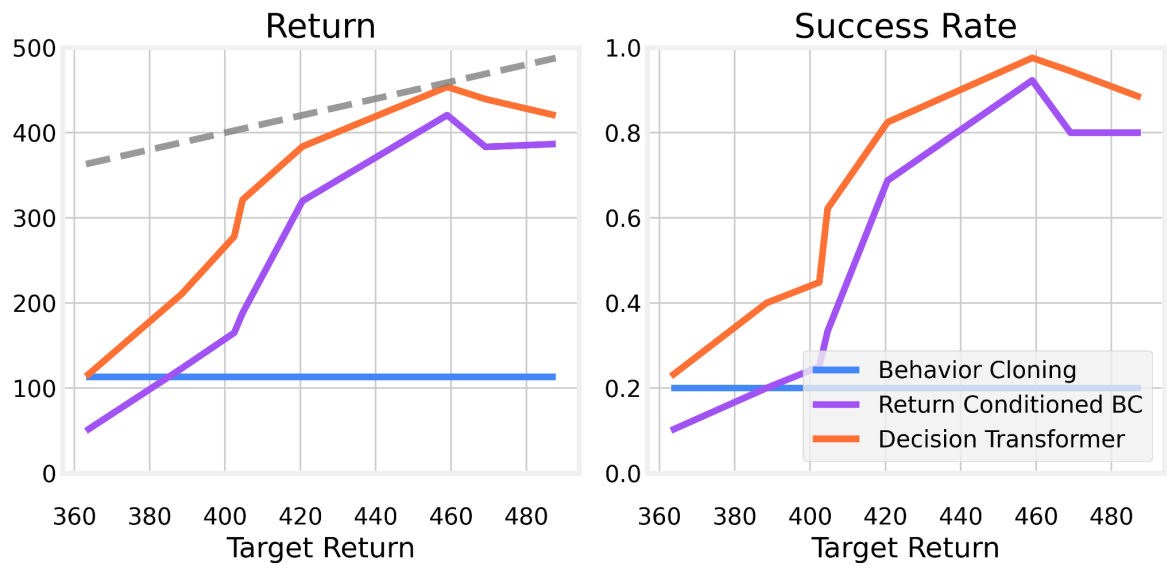
\includegraphics[width=\columnwidth]{figs/success_rate_curve.png}
    \caption{Return-conditioned policies replicate a range of performance qualities. As the target return increases, so does the actual return and success rate of the agents.} 
    \label{fig:success_rate_curve}
\end{figure}

\section{Discussion and Future Work}
\label{sec:discussion}
Our experiments suggest that return-conditioned imitation learning methods like Decision Transformers can outperform standard Behavioral Cloning when learning from mixed-quality data. However, our implementation of DT still underperforms BC models that use the highest quality subset of the dataset (PH). The real promise of Decision Transformer is its ability to mimic high-quality data while still learning whatever may be useful from a large quantity of sub-optimal demonstrations. Ideally, DT would strictly outperform the BC-PH baselines and make use of MG datasets in more difficult robomimic tasks like Square and Tool Hang. We offer three possible explanations for why we are not seeing these results, and suggest directions for future improvement.

First, limited computational resources have restricted our ability to perform large hyperparameter sweeps. It is possible that there are higher-performance model architectures, regularization settings, and other empirical details that could improve our results. We hope that our open-source code release will be a useful starting point for future experiments.

Second, there may be alternative reward functions that are more suitable for return-conditioned BC than the time-based completion bonus used in our experiments (Eq. \ref{eq:rt}). Rewarding the agent for the time to completion clearly separates poor MG demonstrations from quality PH ones. However, it may over-emphasize fast solutions instead of consistent and easily repeatable behavior. Furthermore, the time-based rewards may be too difficult for the sequence model to imitate precisely because it is difficult to identify the current time with a fixed-length context window. Results such as Fig. \ref{fig:success_rate_curve} show that current policies struggle to imitate low-return (slow) demonstrations. We plan to add a timestep counter to the state representation in the open-source release and re-evaluate on the more difficult robomimic tasks.

Finally, there may be meaningful algorithmic changes needed to address some limitations of return-conditioned imitation learning in the robomimic setting. Because the robomimic datasets contain much more machine-generated data than human demonstrations, our return-to-go labeled dataset is heavily skewed toward low-return outcomes. Relabeling trajectories in hindsight with their achieved return creates an implicit ``task-averaging" or return-agnostic term in the resulting policy, which can be especially problematic in cases where the outcome distribution is biased. For more on this issue, we refer the reader to \citep{eysenbach2022imitating}.




\section{Conclusion}

In this paper, we propose a modified version of the Decision Transformer for robotic imitation learning and evaluate its performance on sub-optimal datasets. We show that the Transformer's ability to understand context and long-term dependencies can improve action predictions and outperform return-conditioned behavioral cloning. However, we also find that conditioning on a history of previous actions and RTG scalars can hinder the model's performance and result in distributional shifts during evaluation. We demonstrate that increasing model size can improve performance on both tasks and that longer context sequence lengths can improve prediction accuracy during training. When compared to simpler baselines, we see clear improved performance on both tasks.

Our work has the potential to be applied in various robotics tasks, particularly those that involve working with sub-optimal or ``noisy" data. General robotics research focuses on designing robots that can operate in unstructured environments, such as homes and offices, where data collection for manipulation tasks can be noisy and difficult. Our approach could potentially be a useful starting point for using Decision Transformers to improve the performance of robots in these types of settings. For instance, we can use past versions of data to improve our models over time, employ a wide range of policies on different data types, and reduce the need for extensive data cleaning before training. Additionally, future work should focus on mitigating the distributional shifts observed in our approach and exploring ways of improving the reward function to better support dense rewards. We open-source the entire project as a stepping stone in these endeavors. 



\bibliographystyle{plainnat}
\bibliography{references}

\end{document}


